%!Tex Root = ../Tutorat2.tex

\section{Exercise sheet 2}

\setcounter{task}{1}

\begin{frame}{TT Cyclic Executive Scheduling}{Why scheduling?}
    \begin{itemize}
        \item In many embedded systems, correct timing is a matter of \textbf{correctness}, not performance.
        \item Hard real-time systems can be often found in safety-critical applications. If an answer arrives too late within such a system, the consequences can be a \textbf{catastrophe}.
        \item We want to analyse our systems under a worst case assumption. We need to prove that our system can meet certain deadlines \textbf{reliably} and \textbf{without} statistical arguments.
        \item Given tasks and their deadlines, we now want to find a suitable arrangement of these periodic tasks such that the system can process them while keeping all their constraints in mind. (Or if not possible, we want to find out why not!)
    \end{itemize}
\end{frame}

\begin{frame}{TT Cyclic Executive Scheduling}{Recap: Definitions}
    \begin{itemize}
        \item $\Gamma:$ set of all periodic tasks
        \item $\tau_i:$ one particular periodic task (the i-th)
        \item $\tau_{i,j}:$ the $j$th instance of task $i$
        \item $r_{i,j}:$ release time of $j$th instance of task $i$
        \item $d_{i,j}:$ absolute deadline of the $j$th instance of task $i$
        \item $\Phi_i:$ phase of task $i$
        \item $D_i:$ relative deadline of task $i$
    \end{itemize}
\end{frame}

\begin{frame}{TT Cyclic Executive Scheduling}{Recap: Definitions}
\begin{figure}
    \centering
    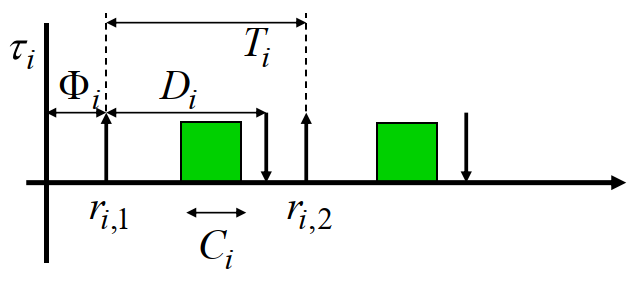
\includegraphics[scale=0.5]{figures/task_instance.png}
    \caption{View on a single task}
    \label{instanceView}
\end{figure}
\end{frame}

\begin{frame}{TT Cyclic Executive Scheduling}{Recap: Three assumptions}
\begin{enumerate}
    \item The instances of a periodic task are regularly activated at a constant rate. The interval between two consecutive activations is called period. The release times satisfy $r_{i,j} = \Phi_i + (j-1)T_i$
    \item All instances have the same worst case execution time $C_i$ (also written as $WCET(i)$)
    \item All instances of a periodic task have the same relative deadline $D_i$. Therefore the absolute deadlines satisfy $d_{i,j} = \Phi_i + (j-1)T_i + D_i$
\end{enumerate}
\end{frame}

\begin{frame}{TT Cyclic Executive Scheduling}{Example Schedule}
Given $P = 12$ and $f = 4$. Given the table below, find a possible frame assignment
\begin{center}
    \begin{tabular}{|c||c|c|c|c|c|}
    \hline
    $\Gamma$ & $T_i$ & $\Phi_i$ & $D_i$ & $C_i$ & frame\\
    \hline
    $\tau_1$ & 12 & 2 & 8 & 2.8 & \\
    \hline
    $\tau_2$ & 12 & 3 & 9 & 3 &\\
    \hline
    $\tau_3$ & 4 & 0 & 4 & 1 &\\
    \hline
\end{tabular}
\end{center}
\end{frame}

\begin{frame}{TT Cyclic Executive Scheduling}{Example Schedule}
\begin{center}
    \begin{tabular}{|c||c|c|c|c|c|}
    \hline
    $\Gamma$ & $T_i$ & $\Phi_i$ & $D_i$ & $C_i$ & frame\\
    \hline
    $\tau_1$ & 12 & 2 & 8 & 2.8 & 2\\
    \hline
    $\tau_2$ & 12 & 3 & 9 & 3 & 3\\
    \hline
    $\tau_3$ & 4 & 0 & 4 & 1 & 1, 2, 3\\
    \hline
\end{tabular}
\end{center}
\begin{figure}
    \centering
    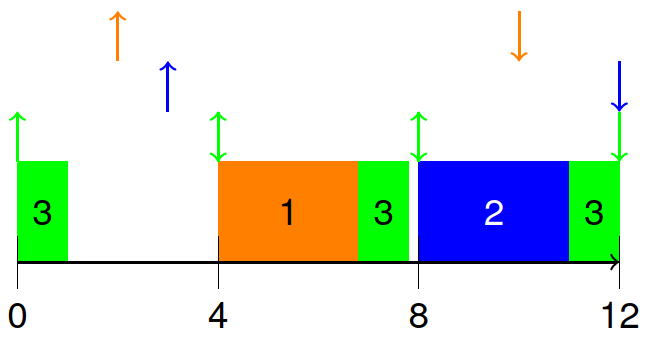
\includegraphics[scale=0.25]{figures/schedule_example.png}
    \caption{Solution}
    \label{exampleSolution}
\end{figure}
\end{frame}

\begin{frame}{TT Cyclic Executive Scheduling}{Exercise 1: Correctness of a Schedule}
In exercise 1 of sheet 2 you are asked to determine the feasability of a given schedule. For this, you need to consider the several questions raised in the lecture:
\begin{enumerate}
    \item Is $P$ a multiple of all periods $T_i$? Is $P$ a multiple of $f$?
    \item Is the frame sufficiently long? $\sum\limits_{\{i\ |\ f_{ij}=k\}}C_i \leq f \qquad \forall 1 \leq k \leq \frac{P}{f}$
    \item Determine offsets such that instances of tasks start after their release time: $\Phi_i = \min\limits_{1\leq j\leq P/T_i} \{(f_{ij}-1)f-(j-1)T_i\} \qquad \forall tasks \ \tau_i$
    \item Are deadlines respected? $(j-1)T_i + \Phi_i + D_i \geq f_{ij}f \quad \forall tasks\ \tau_i,\ 1 \leq j \leq P/T_i$
\end{enumerate}
\end{frame}

\begin{frame}{TT Cyclic Executive Scheduling}{Exercise 2: Finding a Schedule}
In exercise 2 of sheet 2 you are asked to determine a feasible schedule. For this, you need to determine $P$ and $f$ given all the constraints as shown in the lecture to fill every frame. Exercise 3 is the same task and meant as a bonus exercise for those that want more practice.
\end{frame}
